\def\MWS{\textsf{MathWebSearch}\xspace}

\ednote{TW:  Write a general notebook introduction, cite D4.2, D4.3}

\subsection{Formula Search Engine}

\ednote{TW: Change the spin of this entire section as "demos were held together with a lot of effort and duct tape}

\begin{newpart}{from D6.1}

MWS is a web application that provides low-latency answers to full-text queries which consist of keywords and formulae.
\MWS front-ends convert formula schemata (with query variables) into content MathML expressions, which the \MWS formula indexer answers by unification and combines the results with keyword results from a text search engine.
The modular architecture and standardized formats in principle make \MWS applicable to a wide range of querying tasks:
web-based formula search engines or editing support services. 
Unification queries over content MathML expressions form the basis of an expressive query language with well-defined semantics.

We do not give an overview of the pre-existing \MWS architecture here; instead we describe our re-worked design in Section~\ref{sec:software:deployment} below. 
We furthermore refer the interested reader to a more detailed description of the pre-existing system in \ednote{TW: Cite D6.1}. 

The \MWS system has been used to supply search instances on various corpora of mathematical documents, we describe three here, others can be seen on \url{http://search.mathweb.org}. 

\subsubsection{arXiv search}

Begun on August 14, 1991, created by Paul Ginsparg, the ``Cornell e-Print arXiv''
(\url{http://arXiv.org}) is a repository of scientific papers and electronic preprints in
fields of mathematics, computer science, physics, astronomy, biology and statistics or
finance written in {\TeX/\LaTeX} for an optimized transfer over the internet and an easily
rendered client-side. In present the project is hosted by Cornell University and includes
over a million articles and increases with around 8000 per month.

The KWARC group have converted by arXiv corpus into HTML5~\cite{StaKoh:tlcspx10} and
harvested it for \MWS. The instance at \url{http://arxivsearch.mathweb.org}
indexes over 105\,000 math-heavy papers. This subcorpus has also been used for the NTCIR
Math Information Retrieval
Challenges~\cite{AizKohOun:nmpto13,AizKohOunSch:nmto14,AizKohOunSch:nmto16}.

\subsubsection{zbMATH search}

Zentralblatt Math (zbMath) is a mathematical information service that curates a database of reviews and classifications (MSC, see~\cite{MSC2010}) for all articles in mathematics since the middle of the 19th century. The database currently contains 3.8 million reviews and grows at a rate of ca 120\,000 reviews per year.
The zbMATH portal at \url{https://zbmath.org/} offers a faceted search engine for reviews based on bibliographic metadata, MSC classification, and \emph{formulae}.
The latter is driven by \MWS. 

\end{newpart}

\subsection{Enabling Formula Search Deployments}\label{sec:software:deployment}

To use MathWebSearch inside OpenDreamKit, we need to be able to flexibly use it as a new component. 
To achieve this, we developed deployment infrastructure in the form of several components on top of the core MathWebSearch daemon. 
Each component typically exists as a single Docker Container\ednote{TW:  Reference other ODK Docker stuff here}. 
The components are composed using a Docker Compose file.
The structure of our infrastructure can be seen in Figure~\ref{fig:mwsdeployment}. 

\begin{figure}[ht]
  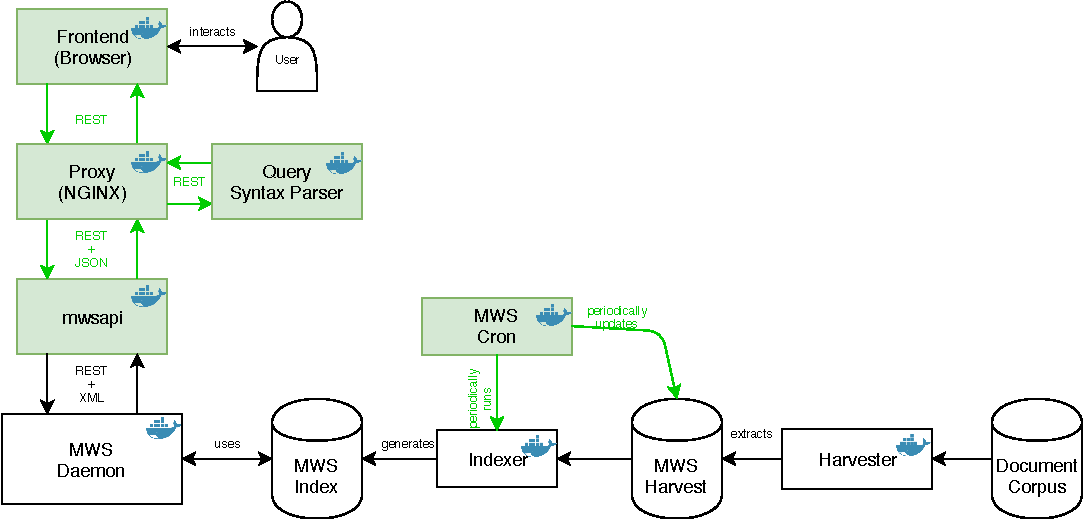
\includegraphics[width=0.8\textwidth]{mws_layout.pdf}
  \caption{Structure of our newly developed MathWebSearch Deployment Infrastructure. Newly developed and updated components colored in green. }\label{fig:mwsdeployment}
\end{figure}

We describe the components of our infrastructure. 

\paragraph{The MathWebSearch Daemon}
The central component is the \textit{MathWebSearch daemon}, which can be found in the bottom left. 
As previously, it uses an \textit{Index} and exposes an XML-based API for queries. 
The only change we made to the core daemon is that it now exists inside a Docker Container. 

\paragraph{The Harvesters and The Indexer}
In order to generate an index from a set of documents, as before, we need two components. 
First we extract a set of ContentMathML formulae using a corpus-specific \textit{Harvester} (bottom right). 
The generated \textit{Harvest} is then sent to the \textit{Indexer} (bottom center), which generates or updates the \textit{Index}. 

Additionally, we introduced a scheduler component called \textit{MWS cron}. 
This periodically sends updated harvests to the \textit{indexer}, which then in turn updates the index. 
This process ensures that the Index remains up-to-date. 

\paragraph{Frontend, mwsapi and the query syntax parser}

In order to process end user queries, we introduced several additional components.

The most important component of these is the \textit{frontend}, which runs inside the users' browser. 
It allows users to enter a formula search query, and view the results. 
The frontend contains corpus-specific branding and text, and is otherwise not corpus-specific. 
In particular the querying code which interacts with the backend components, does not require specialization. 
\ednote{TW:  Screenshot here?}

While the MathWebSearch daemon only understands formulae in Content MathML, users often enter them using different representations, such as \LaTeX. 
For this purpose, the frontend allows entering queries in human-writable, corpus-specific syntax. 
In order to transform the user query into a system-understood query, we make use of a new component called the \textit{Query Syntax Parser}. 
For {\LaTeX} syntax this is achieved using {\LaTeX}ML along with a custom MathWebSearch extension, but this component is fully interchangeable if the user desires other syntaxes. 

The frontend does not directly send MathML queries to the \textit{Daemon}.
Instead, it sends them to a thin API layer on top called \textit{mwsapi}. 
This layer forwards the queries to the daemon and, upon receiving a response, performs some post-processing. 
This process includes transforming substitutions returned by MathWebSearch into a format that can be directly presented to the user by the frontend. 

As the frontend, the mwsapi server and the Query Syntax Presenter are all exposed to the end-user under the same url, a proxy delegating requests accordingly was also neccessary. 
This is using an nginx \ednote{TW: cite} server. 

\subsection{Building a Notebook Search}

For certain situations Sage can produce \LaTeX formulae as output. 
To enable search on these formulae, we developed a harvester and used it in our MathWebSearch infrastructure. 

The harvester takes as input a single Sage Jupyter Notebook, and produces a MathWebSearch Harvest of ContentMathML formulae. 
It achieves this by processing each individual LaTeX formula using LaTeXML. 
We then connected this harvester to the GitHub API and used it to harvest formulae from \ednote{TW: conceptually all, but this part isn't fully fleshed out, hence at the moment only a subset} Sage Jupyter Notebooks on GitHub. 

\ednote{TW: 
yet to do:
- deployed this using customized branding
- screenshot + url
- evalutation: this was easy to do and gave a large benefit to the community
}

\subsection{Future Plans for MathWebSearch}

- describe the custom component / frontends for NLAB
- temasearch
- python ast search + input syntax?

%%% Local Variables:
%%% mode: latex
%%% mode: visual-line
%%% fill-column: 5000
%%% TeX-master: "report"
%%% End:

%  LocalWords:  ednote textbf fig:mwsdeployment includegraphics textwidth mws_layout.pdf textit mwsapi specialization nginx Jupyter customized evalutation temasearch
